%\documentclass[12pt,handout]{beamer}
\documentclass[presentation]{beamer}
\usepackage{../oop-slides-lab}

\usepackage{minted}
\setbeamertemplate{bibliography item}[text]

\newcommand{\lab}{Lab09}

\title[{\lab} -- DVCS Workflow]{Rudimenti di\\Ingegneria del processo di produzione software}

\date[\today]{\today}

\begin{document}

\frame[label=coverpage]{\titlepage}

%====================
%Outline
%====================
\begin{frame}<beamer>
 	\frametitle{Outline}
 	\tableofcontents[]
\end{frame}

\section{DVCS Workflow}

\fr{Dalle puntate precedenti} {
	\bl{DVCS} {
		\iz {
			\item DVCS sono strumenti potenti per tenere traccia in maniera efficiente della storia di un progetto
			\item Nascono in particolare come evoluzione dei tradizionali VCS (SVN, CVS \dots)
			\item Enfasi su una \textbf{miglior gestione del lavoro di team}
		}
	}
	\bl{DVCS e teamwork} {
		\iz {
			\item ``La potenza \`e nulla senza controllo!''
			\item Ovvero \dots la mancanza di un metodo chiaro e condiviso per utilizzarli può portare a risultati \textbf{DEVASTANTI}
            \iz {
                \item effort necessario per la parte di gestione diventa presto preponderante e insostenibile
            }
			\item Ecco perché è bene adottare un \textbf{workflow collaborativo}
            \iz {
                \item i vostri progetti e i vostri partner di progetto vi ringrazieranno!
            }
		}
    }
}

\fr{Quale workflow} {
        \iz {
			\item Come si sceglie un workflow?
            \item Abbiamo parlato di semplicità...
            \item In realtà è più corretto parlare di giusto \textbf{trade-off} tra semplicità ed esigenze
		}
}

\fr{Lo stato dell'arte I} {
Definito da \emph{Vincent Driessen} e spiegato in \url{http://nvie.com/posts/a-successful-git-branching-model/}
\begin{center}
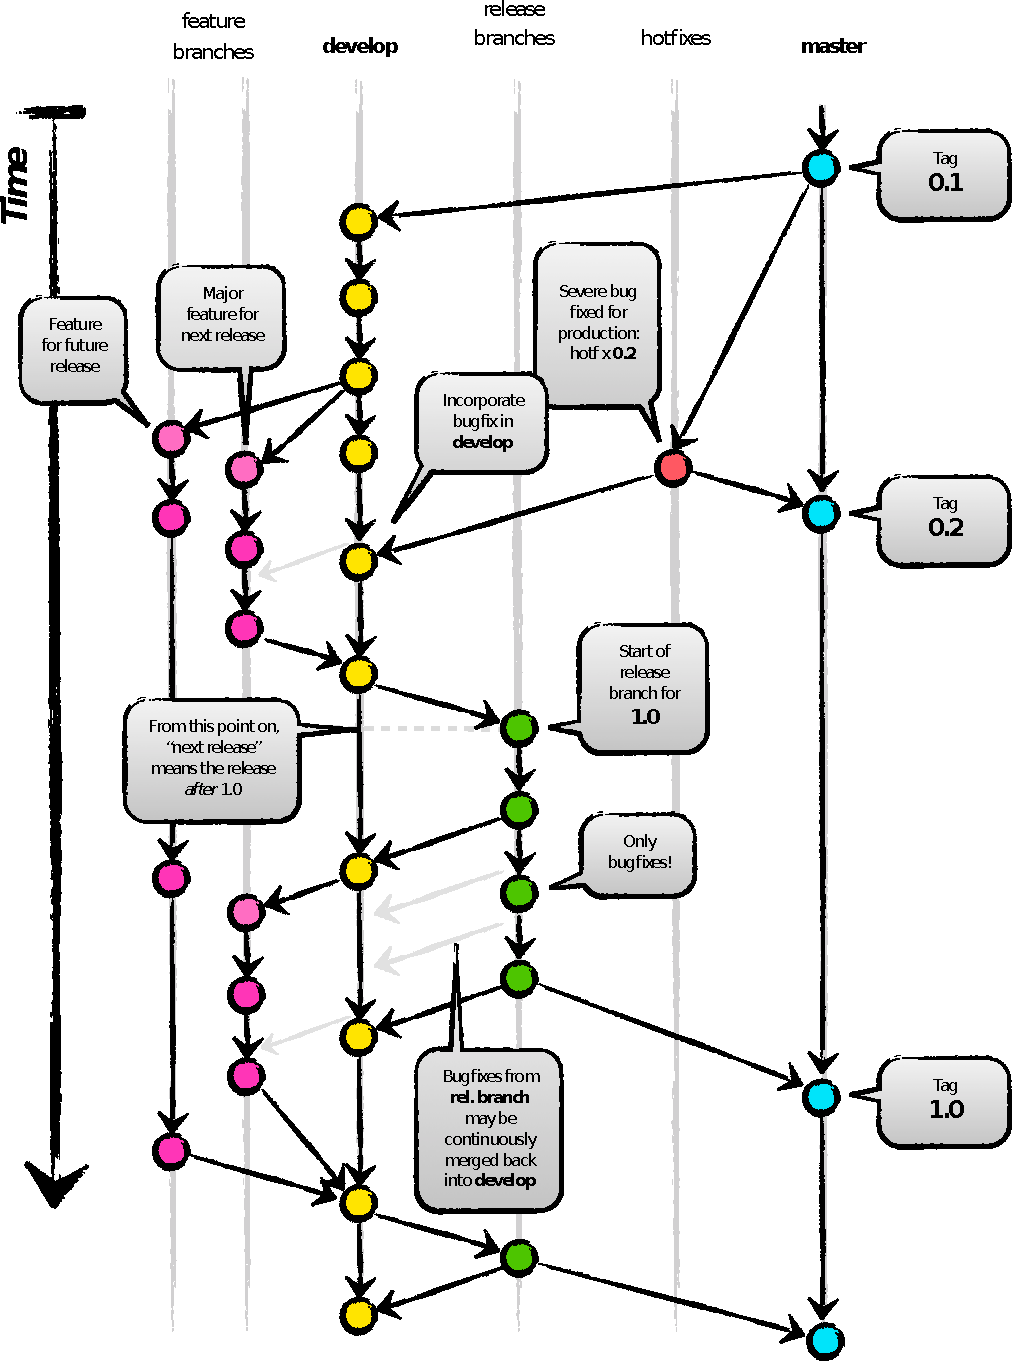
\includegraphics[width=0.4\textwidth]{img/Git-branching-model}
\end{center}
}

\fr{Lo stato dell'arte II} {
    \bl{Alcune considerazioni} {
        \iz {
			\item Non lo useremo
            \iz{
                \item troppo complicato per i nostri scopi
            }
            \item Comunque molto interessante perché racchiude tutti gli aspetti di un DVCS workflow
        }
    }

    \bl{I branch} {
		\iz {
			\item Sono il supporto fondamentale alle fasi del ciclo di vita del software
			\item Ogni fase ha il proprio branch!
			\item Branching e merging all'ordine del giorno!
		}
	}
}


\fr{Un modello più semplice} {
    \begin{center}
        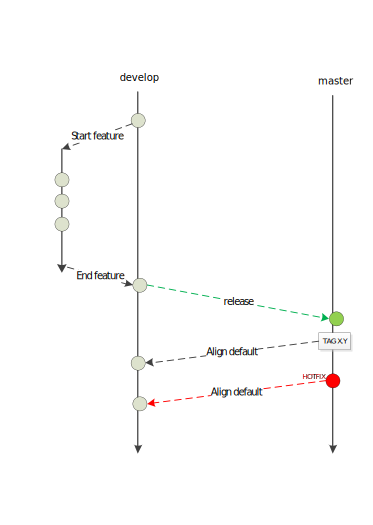
\includegraphics[width=0.5\textwidth]{img/visio-workflow-mercurial}
    \end{center}
}

\begin{frame}[fragile, allowframebreaks]{Feature branch}
	\begin{center}
		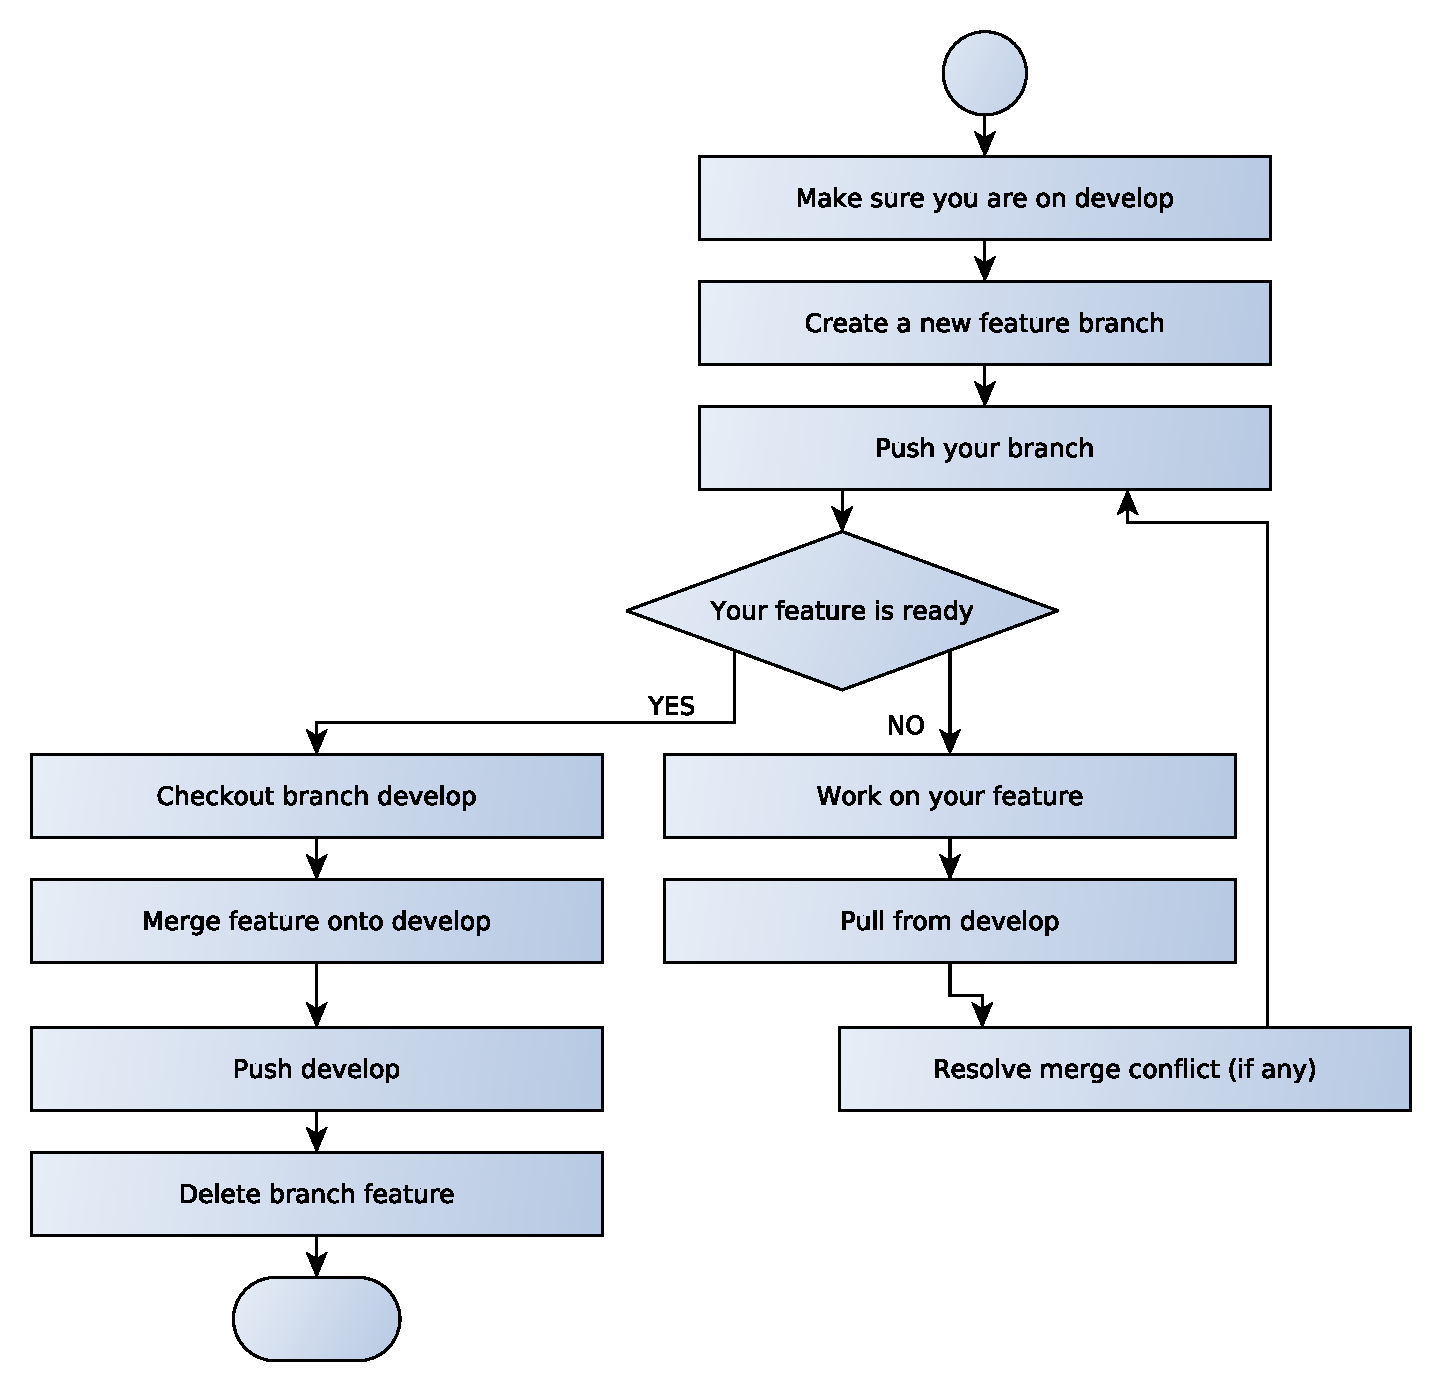
\includegraphics[height=.8\textheight]{img/feature}
	\end{center}
	\sizedcoded{\tiny}{code/open-feature.txt}{language=bash}
\end{frame}

% \subsection{Comandi}
%
% \fr{Inizializzazione del repository} {
% \sizedcode{\tiny}{code/init.txt}
% }

%
% \begin{frame}[allowframebreaks]{Associazione di nomi simbolici ad un commit}
% 	\bl{In generale}{
% 		È necessario poter associare ad un commit della meta-informazione personalizzata. Ad esempio, per associare un certo commit ad una versione, in modo da poterla facilmente richiamare.
% 	}
% 	\bl{In Git}{
% 		\iz{
% 			\item \texttt{git tag -a MyTag -m "My tag information"}
% 			Associa al commit corrente il nome simbolico \texttt{MyTag} ed il messaggio aggiuntivo \texttt{My tag information}
% 			\begin{itemize}
% 				\item Non rimpiazza il commit message, ma lo integra
% 				\item È possibile invocare comandi come \texttt{git checkout MyTag} per tornare velocemente ad un tag precedente
% 			\end{itemize}
% 			\item \texttt{git push --tags}
% 			\begin{itemize}
% 				\item Fa \texttt{push} delle metaiformazioni aggiunte col comando \texttt{tag}
% 				\item La \texttt{push} ``normale'' non invia queste informazioni!
% 			\end{itemize}
% 		}
% 	}
% \end{frame}
%
%
%
% \fr{Fare una release} {
% \sizedcode{\tiny}{code/do-release.txt}
% }

\begin{frame}[allowframebreaks]{Il repo ufficiale del vostro progetto}
	\begin{block}{Workflow raccomandato}
		\begin{itemize}
			\item Qualcuno di voi agirà come ``repo maintainer''
			\item Creerà quindi il repository su GitHub
			\item Gli altri membri del team faranno la \texttt{clone}
			\item Ciascuno lavorerà parallelamente sul proprio repository locale (working copy), condividendo tramite \texttt{push} e \texttt{pull} il proprio lavoro con gli altri
		\end{itemize}
	\end{block}
	\begin{block}{Workflow avanzato}
		Ottimo per progetti di grosse dimensioni e/o per team molto eterogenei, dove qualcuno deve assicurarsi della qualità del codice prodotto da altri.
		\begin{itemize}
			\item Il maintainer crea il repository, ed è l'unico col diritto di scrittura
			\item Gli altri membri del team hanno una fork a testa
			\item Ciascuno lavora su una working copy, facendo pull dal repository ``centrale'' e push sulla propria fork
			\item Quando una feature è completa, o si arriva ad un buon grado di sviluppo, si apre una \textbf{pull request}
			\item Il maintainer revisiona il codice, assegna eventuali modifiche, e quando è soddisfatto accetta la pull request facendo il merge del codice nel repository principale
		\end{itemize}
		Questo workflow è un overkill per il progetto di OOP
		\begin{itemize}
			\item Ma è possibile che vi chiederemo di lavorare così, se farete tesi o un tirocini relativi ad alcuni nostri software
		\end{itemize}
	\end{block}
\end{frame}

\section{Rudimenti di Gradle}

\subsection{Gestione delle dipendenze}

\begin{frame}[fragile]{Mini challenge}
\begin{block}{}
Scrivere un programma che va su Internet, scarica da TheTVDB i titoli degli episodi di Breaking Bad in italiano, e poi li stampa.
\end{block}

\pause
\begin{minted}[fontsize=\tiny,linenos=true,breaklines=true]{java}
package it.unibo.ci;
import java.io.IOException;
import org.apache.commons.io.IOUtils;
import com.omertron.thetvdbapi.TheTVDBApi;
import com.omertron.thetvdbapi.model.Episode;
import com.omertron.thetvdbapi.model.Series;
import static java.nio.charset.StandardCharsets.UTF_8;

public final class PrintBreakingBad {
    private static final String LANG = "it";
    private static final String SERIE = "Breaking Bad";
    private PrintBreakingBad() { }
    public static void main(String... args) throws ClassNotFoundException, IOException {
        final var externalKeyFile = ClassLoader.getSystemResourceAsStream("TheTVDBAPIKey")
        final var key = IOUtils.toString(externalKeyFile, UTF_8);
        final var api = new TheTVDBApi(key);
        api.searchSeries(SERIE, LANG).stream()
            .filter(s -> s.getSeriesName().equals(SERIE))
            .map(Series::getId)
            .flatMap(s -> api.getAllEpisodes(s, LANG).stream())
            .map(Episode::getEpisodeName)
            .forEach(System.out::println);
    }
}
\end{minted}
\end{frame}

\begin{frame}{Librerie}
    Sono state usate due librerie:
    \begin{itemize}
        %\item Google Guava (\texttt{com.google.guava:guava})
        \item Apache Commons IO (\texttt{commons-io:commons-io})
        \item Omertron's TheTVDBApi (\texttt{com.omertron:thetvdbapi})
    \end{itemize}
    ...solo che per far funzionare TheTVDBApi servono altre due librerie...
    \begin{itemize}
        \item SLF4J (\texttt{org.slf4j:slf4j-api})
        \item YAMJ (\texttt{org.yamj:api-common})
    \end{itemize}
    ...solo che per far funzionare YAMJ servono altre sei librerie...

    ...e per far funzionare alcune di queste servono altre librerie ancora
\end{frame}

\begin{frame}[fragile]{Albero delle dipendenze}
    Si crea un \textit{albero} delle dipendenze!

%+--- com.google.guava:guava:19.0-rc2
    \begin{minted}[fontsize=\scriptsize]{text}
+--- commons-io:commons-io:2.4
\--- com.omertron:thetvdbapi:1.7
     +--- org.slf4j:slf4j-api:1.7.9
     \--- org.yamj:api-common:1.2
          +--- org.apache.commons:commons-lang3:3.3.2
          +--- commons-dbcp:commons-dbcp:1.4
          |    \--- commons-pool:commons-pool:1.6
          +--- commons-pool:commons-pool:1.6
          +--- commons-codec:commons-codec:1.10
          +--- org.apache.httpcomponents:httpclient:4.3.6
          |    +--- org.apache.httpcomponents:httpcore:4.3.3
          |    +--- commons-logging:commons-logging:1.1.3
          |    \--- commons-codec:commons-codec:1.10
          \--- org.slf4j:slf4j-api:1.7.9
    \end{minted}
    \begin{itemize}
        \item La gestione manuale può diventare dispendiosa
        \begin{itemize}
            \item Ad ogni aggiornamento bisogna ricontrollare tutto il sotto-albero
        \end{itemize}
        \item Le dipendenze indirette (\textit{transitive}) potrebbero avere versioni confliggenti!
    \end{itemize}
\end{frame}

\begin{frame}[fragile]{Contesti delle dipendenze}
    Non è il solo problema
    \begin{itemize}
        \item Alcune dipendenze ci servono solo a runtime, non a compile time
        \item Alcune dipendenze ci servono solo per il testing (JUnit ad esempio)
    \end{itemize}
    Andrebbero creati diversi classpath, uno per ``scope'':
    \begin{itemize}
        \item implementazione (compilazione ed esecuzione)
        \begin{itemize}
            \item per il prodotto
            \item per i test
        \end{itemize}
        \item solo compilazione (no runtime)
        \begin{itemize}
            \item per il prodotto
            \item per i test
        \end{itemize}
        \item solo esecuzione (no compilazione)
        \begin{itemize}
            \item per il prodotto
            \item per i test
        \end{itemize}
    \end{itemize}
    ...i problemi cominciano a sommarsi...
\end{frame}

\begin{frame}{Gradle}
    Build automation tool: automatizza la gestione del progetto
    \begin{itemize}
        \item Gestione delle dipendenze
        \begin{itemize}
            \item Cerca le librerie
            \item Le scarica
            \item Prepara il classpath
        \end{itemize}
        \item Build automation
        \begin{itemize}
            \item Compila il progetto ed i test
            \item Genera i jar
            \item Genera la documentazione
        \end{itemize}
        \item Controllo qualità
        \begin{itemize}
            \item esegue i test
            \item verifica la qualità del codice
        \end{itemize}
        \item Deployment
    \end{itemize}
\end{frame}

\begin{frame}[allowframebreaks]{Gradle: configurazione}
    \begin{itemize}
        \item La build è definita all'interno di un file \texttt{build.gradle.kts}
        \begin{itemize}
            \item Scritto in Kotlin
            \item Oppure in Groovy (cambia nome in \texttt{build.gradle})
        \end{itemize}
        \item Sfrutta il principio \textbf{Convention over Configuration}
        \begin{itemize}
            \item Ho un funzionamento di default
            \item Se fai le cose come me le aspetto non devi dirmi nulla
            \item Ogni cosa diversa va configurata
        \end{itemize}
        \item Supporta vari linguaggi
        \begin{itemize}
            \item Fra cui Java
        \end{itemize}
        \item Estensibile tramite plugin
    \end{itemize}
\end{frame}

\begin{frame}[fragile]{Gradle + Java}
Configurazione per il nostro esperimento:
\begin{block}{}
\begin{minted}[fontsize=\small,linenos=true,breaklines=true]{kotlin}
plugins {
    java
}
repositories {
    mavenCentral() // Where to look for jars
}
dependencies {
    implementation("commons-io:commons-io:2.4")
    implementation("com.omertron:thetvdbapi:1.7")
    testImplementation("junit:junit:4.12")
}
\end{minted}
%implementation("com.google.guava:guava:19.0-rc2")
\end{block}
\begin{itemize}
    \item Se importato in Eclipse come ``Gradle Project'' scarica automaticamente i jar necessari e li mette nel classpath!
\end{itemize}
\end{frame}

\begin{frame}[fragile]{Convenzioni Java in Gradle}
    A meno di non usare configurazione manuale, Gradle si aspetta una struttura un diversa da quella di default in Eclipse
    \begin{itemize}
        \item Chi usasse Gradle, dovrebbe optare per questa convenzione, ed importare il progetto in Eclipse dopo averla applicata
        \item È la convenzione che si usa nei progetti ``seri''
        \item Deriva da uno strumento di build automation antesignano di Gradle (Apache Maven)
    \end{itemize}
    \begin{minted}[fontsize=\small,linenos=true,breaklines=true]{text}
    |-- src
    |   |-- main
    |   |   |-- java          Sorgenti java (ex: src)
    |   |   \-- resources     Risorse del software (ex: res)
    |   \-- test
    |       |-- java          Sorgenti java per i test
    |       \-- resources     Risorse per i test
    \-- build.gradle.kts      Build file
    \end{minted}
\end{frame}

\subsection{Concetti fondamentali}

\begin{frame}[allowframebreaks]{Concetti fondamentali}
    \begin{block}{Progetto}
        L'insieme di cose che volete costruire o fare con Gradle, ed i file che consentono di farlo. Ogni progetto è costituito di uno o più \textit{task}
    \end{block}
    \begin{block}{Task}
        Operazione atomica eseguita sul progetto (ad esempio, compilazione di file Java, o impacchettamento di un jar). Può dipendere da altri task (ad esempio, la creazione di un jar eseguibile richiede che la compilazione dei sorgenti sia stata completata).
    \end{block}
    \begin{block}{Plugin}
        Componente che estende le funzionalità di Gradle, aggiungendo configurazioni e task
    \end{block}
\end{frame}

\begin{frame}{Gradle: funzionamento}
    \begin{itemize}
        \item È possibile chiedere a Gradle di completare un task eseguendo il comando:
        \begin{itemize}
            \item \texttt{gradle nomeTask}
            \item Esegue tutti i task necessari ad eseguire \texttt{nomeTask}, quindi esegue \texttt{nomeTask}
        \end{itemize}
        \item I task esistenti si possono visualizzare con:
        \begin{itemize}
            \item \texttt{gradle tasks --all}
        \end{itemize}
        \item Le dipendenze (anche transitive) possono essere visualizzate con:
        \begin{itemize}
            \item \texttt{gradle dependencies}
        \end{itemize}
    \end{itemize}
\end{frame}

\begin{frame}[allowframebreaks]{Gradle wrapper}
    Problema: ma se cambiassero il modo in cui Gradle risolve le dipendenze?
    \begin{itemize}
        \item Il sistema potrebbe ad un certo punto cambiare delle dipendenze transitive
        \item Il classpath cambierebbe
        \item Potenzialmente il nostro software potrebbe smettere di funzionare!
        \item (nota: è successo davvero...)
        \begin{itemize}
            \item (...svariate volte)
        \end{itemize}
    \end{itemize}
    \begin{center}
        
\includegraphics[width=0.6\textwidth]{img/philosoraptor}
    \end{center}
    Gradle fornisce una funzionalità detta \textbf{wrapper}
    \begin{itemize}
        \item Un piccolo script, contenente solo le informazioni necessarie a scaricare e usare la corretta versione di Gradle
        \item generabile da Gradle tramite il task \texttt{wrapper}
        \begin{itemize}
            \item \texttt{gradle wrapper --gradle-version=X.Y.Z}
        \end{itemize}
        \item dal momento in cui è presente il wrapper, è possibile usare quello per eseguire la corretta versione di Gradle!
        \begin{itemize}
            \item \texttt{./gradlew nomeTask} --- su Unix o emulatore bash come git bash
            \item \texttt{gradlew.bat nomeTask} --- su Windows cmd o Powershell
        \end{itemize}
        \item \textbf{È sempre meglio usare il wrapper!}
        \item Ovviamente è possibile generare il wrapper usando il wrapper:
        \begin{itemize}
            \item \texttt{./gradlew wrapper --gradle-version=X.Y.Z}
        \end{itemize}
        \item Grazie al wrapper, è possibile eseguire Gradle anche se non si ha Gradle installato!
    \end{itemize}
\end{frame}

\subsection{Gradle in OOP}

\begin{frame}[fragile]{Uso raccomandato}
    \begin{itemize}
        \item La costruzione e automazione di un processo di build \textbf{non} è parte della programmazione ad oggetti in quanto tale
        \item È un tema legato all'ingegneria del processo di produzione del software
        \item Molto sfaccettato, fra gli altri include aspetti che vedrete in futuro
        \begin{itemize}
            \item Tecniche agili (e.g. Scrum)
            \item Versioning
            \item Build automation
            \item Continuous integration
            \item Continuous delivery
            \item Deploy automation
            \item ...
        \end{itemize}
        \item La competenza con Gradle acquisibile da OOP è rudimentale
    \end{itemize}
    \begin{center}
        \underline{\textbf{Consiglio:} usate Gradle come semplice gestore di dipendenze}
    \end{center}
\end{frame}


\section{Preparazione al laboratorio}

\begin{frame}{Modalità di lavoro}
	\begin{enumerate}
		\item Forkare e clonare il repository fornito
		\item Seguire le istruzioni nel file \texttt{README.md} nella root del repository
		\item Leggere attentamente le istruzioni e risolvere l'esercizio in autonomia
		\begin{itemize}
			\item Contattare il docente se si rimane bloccati
		\end{itemize}
		\item Utilizzare i metodi \texttt{main} e/o i test per verificare la correttezza delle soluzioni
		\item Cercare di risolvere autonomamente eventuali piccoli problemi che possono verificarsi durante lo svolgimento degli esercizi
		\begin{itemize}
			\item Contattare il docente se, anche dopo aver usato il \textbf{debugger}, non si è riusciti a risalire all'origine del problema
		\end{itemize}
		%\item \textcolor{red}{Scrivere il Javadoc per l'esercizio svolto}
		\item Effettuare almeno un commit ad esercizio completato
		\begin{itemize}
			\item Fatene pure quanti ne volete durante l'esercizio stesso
		\end{itemize}
		\item \textbf{A esercizio ultimato sottoporre la soluzione al docente/tutor}
		\item Proseguire con l'esercizio seguente
	\end{enumerate}
\end{frame}


\end{document}

